\section{Conditional reconstruction and comparison protocol}
\label{sec:supp-protocol}
The main comparison reconstructs scenes under supplied camera and actor states. The last four frames evaluate conditional temporal extrapolation. Table~\ref{tab:shared-inputs} lists test conditions. Target human joints come from independent offline annotation/fitting, and human shape and binding are recovered from context. Test LiDAR is reserved for evaluation. All test-time network weights remain fixed.

\paragraph{Training resources.}
We retrain STORM, DGGT, and StreetForward from random initialization, preserving their native architectures. Every method uses the same real training logs $D_R$, synthetic scenes $D_S$, and complete assets $D_A$. Baselines receive RGB, depth, silhouette, and complete-asset target views through their native objectives. Ours additionally uses cell-empty and template-binding supervision. Checkpoints are selected on the shared development set within each fixed training budget (Table~\ref{tab:baseline-resources}). Matching recovery, codec, data, and optimization in the CCM ablation isolates the contribution of component exchange.

\begin{table*}[t]
\centering\small
\caption{Training resources for one complete checkpoint, including method-specific target preprocessing. Ours and w/o CCM include the shared recovery and codec stages.}
\label{tab:baseline-resources}
\begin{tabular}{@{}lp{0.39\textwidth}rrr@{}}
\toprule
Method & Training objective & Updates & Global batch & GPU hours \\
\midrule
STORM & Native reconstruction plus same-source synthetic views & 234,816 & 16 & 916.7 \\
DGGT & Native geometry/rendering plus same-source synthetic views & 212,672 & 16 & 1,128.4 \\
StreetForward & Native scene reconstruction plus same-source synthetic views & 246,144 & 8 & 1,036.9 \\
Ours & Four-stage training & 287,360 & By stage & 1,001.5 \\
w/o CCM & Shared R/C; retrained GCM prior and adaptation & 287,360 & As Ours & 977.1 \\
\bottomrule
\end{tabular}
\end{table*}

\paragraph{Shared state adapter.}
The baselines use a common deterministic state adapter. Visible Gaussian rendering contributions are projected into the same context instance masks and accumulate weighted identity votes. Vehicles are canonicalized with the inverse supplied root SE(3), transforming centers, covariances, and directional coordinate bases together. Human Gaussians obtain 17-joint skinning weights by barycentric interpolation on corresponding triangles of the context-recovered identity template, followed by inverse skinning. The adapter preserves predicted appearance and adds no prediction network. Unbound outputs remain scored, and actor edits that cannot be assembled count as failures.

For the same Gaussian set, inverse and forward placement produce a maximum linear-RGB difference below $4\times10^{-6}$. Converting a native time-varying representation into fixed canonical assets changes cross-time reconstruction as shown in Table~\ref{tab:adapter-effect}. The adapted column is used in the main comparison.

\begin{table}[t]
\centering\small
\caption{Effect of conversion to fixed canonical assets. PSNR is in dB.}
\label{tab:adapter-effect}
\begin{tabular}{@{}lrrr@{}}
\toprule
Method & Native & Adapted & Change \\
\midrule
STORM & 26.492 & 26.380 & $-0.112$ \\
DGGT & 27.538 & 27.410 & $-0.128$ \\
StreetForward & 27.094 & 27.010 & $-0.084$ \\
\bottomrule
\end{tabular}
\end{table}

\begin{table*}[!t]
\centering\small
\setlength{\tabcolsep}{4pt}
\caption{Test conditions shared by DriveCompose, STORM, DGGT, and StreetForward.}
\label{tab:shared-inputs}
\begin{tabular}{@{}lp{0.67\textwidth}@{}}
\toprule
Condition & Shared setting \\
\midrule
Context RGB & The same four timestamps and three cameras \\
Camera and ego state & Shared intrinsics, extrinsics, and ego poses \\
Test depth/LiDAR & Not an input; depth is estimated from RGB \\
Identity, boxes, root tracks & Shared supplied states \\
Human shape and binding & Recovered from context; common binding interface \\
Target human joints & Shared independent offline annotations/fits \\
Test-scene optimization & None for any method \\
\bottomrule
\end{tabular}
\end{table*}

The first 200 valid synchronized frames per test sequence form ten non-overlapping 20-frame clips, totaling 2,020 clips. Context indices are $\{0,5,10,15\}$ for three cameras. Twelve interpolation frames yield 72,720 images, and the four extrapolation frames $\{16,17,18,19\}$ yield 24,240, totaling 96,960 targets. Every target timestamp has valid dynamic masks and depth-evaluation samples. Aggregating Table~\ref{tab:temporal-groups} at a $3{:}1$ interpolation/extrapolation ratio recovers the main-table means. Depth scale alignment is used only for evaluation, with no feedback to reconstruction or rendering.

\begin{table*}[!t]
\centering\small
\setlength{\tabcolsep}{4pt}
\caption{Temporal interpolation and conditional extrapolation. Image columns report PSNR/SSIM; depth reports scale-aligned AbsRel/$\delta_1$.}
\label{tab:temporal-groups}
\begin{tabular}{@{}lcccc@{}}
\toprule
Method & Time group & Full image & Dynamic region & Depth \\
\midrule
STORM & Interp. & 26.800/0.838 & 22.600/0.640 & 0.170/0.753 \\
STORM & Extrap. & 25.120/0.790 & 20.600/0.576 & 0.202/0.705 \\
DGGT & Interp. & 27.800/0.806 & 23.200/0.667 & 0.237/0.680 \\
DGGT & Extrap. & 26.240/0.758 & 21.240/0.603 & 0.285/0.632 \\
StreetForward & Interp. & 27.400/0.830 & 21.500/0.608 & 0.185/0.771 \\
StreetForward & Extrap. & 25.840/0.782 & 19.176/0.544 & 0.233/0.723 \\
Ours & Interp. & \textbf{28.900/0.909} & \textbf{25.500/0.870} & \textbf{0.091/0.885} \\
Ours & Extrap. & \textbf{27.556/0.877} & \textbf{23.700/0.838} & \textbf{0.107/0.853} \\
\bottomrule
\end{tabular}
\end{table*}

\paragraph{Depth scale and metric evaluation.}
The aligned depth columns use a positive per-frame scale on a fixed valid LiDAR mask $M_t$,
\begin{equation}
s_t=\operatorname{median}_{p\in M_t}\frac{d_t(p)}{\widehat d_t(p)}.
\label{eq:depth-alignment}
\end{equation}
Only scale is fitted. Table~\ref{tab:depth-scale} uses the same masks and frame--clip--sequence aggregation for aligned and unaligned depth. Alignment is applied inside the depth evaluator; reconstruction, composition, surface distances, and RGB reprojection use the original metric coordinates.

\begin{table*}[t]
\centering\small
\caption{Depth evaluation with and without per-frame scale alignment.}
\label{tab:depth-scale}
\begin{tabular}{@{}lrrrr@{}}
\toprule
& \multicolumn{2}{c}{Per-frame scale aligned} & \multicolumn{2}{c}{Unaligned} \\
\cmidrule(lr){2-3}\cmidrule(lr){4-5}
Method & AbsRel $\downarrow$ & $\delta_1\uparrow$ & AbsRel $\downarrow$ & $\delta_1\uparrow$ \\
\midrule
STORM & 0.178 & 0.741 & 0.226 & 0.683 \\
DGGT & 0.249 & 0.668 & 0.327 & 0.572 \\
StreetForward & 0.197 & 0.759 & 0.254 & 0.694 \\
Ours & \textbf{0.095} & \textbf{0.877} & \textbf{0.121} & \textbf{0.842} \\
\bottomrule
\end{tabular}
\end{table*}

\section{Ablations, seed statistics, and evaluation denominators}
\label{sec:supp-ablations}
The two learned variants use training seeds $\{0,1,2\}$ and generation seeds $\{7,17,27\}$ for each checkpoint, giving nine combinations. We first average generation seeds, then frames, windows, sequences, and training seeds equally, without best-of-three selection. In Tables~\ref{tab:seed-components} and~\ref{tab:seed-inputs}, each entry is the mean $\pm$ sample SD of the three training-seed means; parentheses give the average sample SD across generation seeds. Zero variation for w/o GCM describes deterministic inference with shared, fixed recovery and codec.

\begin{table*}[!t]
\centering\small
\setlength{\tabcolsep}{4pt}
\caption{Full seed statistics for component ablations.}
\label{tab:seed-components}
\begin{tabular}{@{}lccc@{}}
\toprule
Metric & w/o GCM & w/o CCM & Ours \\
\midrule
Full-image PSNR & 27.137 $\pm$ 0 & 28.286 $\pm$ 0.074 (0.032) & \textbf{28.913 $\pm$ 0.061 (0.028)} \\
Full-image SSIM & 0.867 $\pm$ 0 & 0.893 $\pm$ 0.001 (0.0006) & \textbf{0.911 $\pm$ 0.001 (0.0005)} \\
Full-image LPIPS & 0.183 $\pm$ 0 & 0.147 $\pm$ 0.002 (0.0013) & \textbf{0.129 $\pm$ 0.002 (0.0011)} \\
Dynamic PSNR & 23.431 $\pm$ 0 & 24.683 $\pm$ 0.112 (0.048) & \textbf{25.617 $\pm$ 0.095 (0.041)} \\
Dynamic SSIM & 0.811 $\pm$ 0 & 0.849 $\pm$ 0.002 (0.0010) & \textbf{0.873 $\pm$ 0.002 (0.0008)} \\
\bottomrule
\end{tabular}
\end{table*}

\begin{table*}[!t]
\centering\small
\setlength{\tabcolsep}{4pt}
\caption{Input-timestamp sensitivity with fixed checkpoints; $T=8$ reuses the component results.}
\label{tab:seed-inputs}
\begin{tabular}{@{}lcccc@{}}
\toprule
$T$ & Variant & PSNR $\uparrow$ & SSIM $\uparrow$ & LPIPS $\downarrow$ \\
\midrule
2 & w/o CCM & 25.237 $\pm$ 0.103 (0.055) & 0.817 $\pm$ 0.003 (0.0011) & 0.254 $\pm$ 0.004 (0.0023) \\
2 & Ours & \textbf{26.341 $\pm$ 0.089 (0.047)} & \textbf{0.851 $\pm$ 0.002 (0.0009)} & \textbf{0.213 $\pm$ 0.003 (0.0019)} \\
4 & w/o CCM & 27.126 $\pm$ 0.086 (0.041) & 0.869 $\pm$ 0.002 (0.0008) & 0.187 $\pm$ 0.003 (0.0018) \\
4 & Ours & \textbf{27.864 $\pm$ 0.072 (0.035)} & \textbf{0.891 $\pm$ 0.001 (0.0006)} & \textbf{0.159 $\pm$ 0.002 (0.0014)} \\
8 & w/o CCM & 28.286 $\pm$ 0.074 (0.032) & 0.893 $\pm$ 0.001 (0.0006) & 0.147 $\pm$ 0.002 (0.0013) \\
8 & Ours & \textbf{28.913 $\pm$ 0.061 (0.028)} & \textbf{0.911 $\pm$ 0.001 (0.0005)} & \textbf{0.129 $\pm$ 0.002 (0.0011)} \\
\bottomrule
\end{tabular}
\end{table*}

Each of the 202 test sequences contributes one 29-timestamp window. Inputs $\mathcal T_2=\{0,28\}$, $\mathcal T_4=\{0,8,20,28\}$, and $\mathcal T_8=\{0,4,\ldots,28\}$ share seven target timestamps $\{2,6,\ldots,26\}$ and three cameras, giving 4,242 target images per combination. Two learned variants, three input settings, and nine seed combinations yield 54 groups and 229,068 predictions. The deterministic w/o GCM control adds 4,242, totaling 233,310.

Non-renderable counts are $0/10,908$ learned-variant window instances and $0/202$ for w/o GCM. Low quality, holes, and contact errors remain scored. All variants share preprocessing, $240\times160$ resolution, annotation-based dynamic masks, and equal sequence weighting. Training samples $T\in\{2,4,8\}$ uniformly, and inference uses 24 Euler steps. Hyperparameters are selected only on the development split.
\section{Off-trajectory, hidden-region, and context diagnostics}
\label{sec:supp-hidden}
Each offset direction renders $2,020\times3\times20=121,200$ images and 6,060 videos. Videos contain 20 frames at 10 Hz and never concatenate clips. The reference population consists of original-trajectory recordings from the same test clips, cameras, and timestamps. FID uses a fixed Inception-v3 with 2,048-dimensional features; FVD uses a fixed I3D with 1,024-dimensional features. Left and right scores are computed separately and averaged, without pooling the two populations first. GT in the main off-trajectory figure denotes the original-trajectory image.

One hundred synthetic test scenes separately provide paired evaluation of regions never observed in the inputs (Table~\ref{tab:hidden-regions}), using representative shifts of $\pm2$ m. FID/FVD describe distribution quality, whereas hidden-region metrics evaluate scene-corresponding completion.


\paragraph{Predicted surfaces and geometry metrics.}
We construct surfaces by rendering and fusion. Gaussians with opacity at least 0.01 are evaluated within $3\sigma$. Six axis-aligned orthographic views are rendered in blocks over a common evaluation domain, with pixel size at most 1 mm inside each block. A ray's first accumulated-opacity crossing of 0.5 defines a surface depth; rays below this opacity have no predicted surface. We fuse depths into a sparse TSDF with 2 mm voxels and an 8 mm truncation distance, and extract the mesh in valid, supported voxels, leaving unknown regions open. Native neural fields use the same accumulated-opacity threshold, fusion, and distance evaluation.

Predicted and reference meshes each supply 65,536 area-uniform samples. A BVH computes each sample's nearest distance to the other triangle mesh. Coordinates are in meters and distances are non-squared Euclidean distances. Evaluation keeps the original metric scale and alignment. With predicted samples $P$, reference samples $G$, and corresponding surfaces $S_{\rm pred}$ and $S_{\rm GT}$ in the evaluation region,
\begin{align}
P_\tau&=\frac{1}{|P|}\sum_{p\in P}\mathbf1[d(p,S_{\rm GT})<\tau],\\
R_\tau&=\frac{1}{|G|}\sum_{g\in G}\mathbf1[d(g,S_{\rm pred})<\tau],\\
F_\tau&=\frac{2P_\tau R_\tau}{P_\tau+R_\tau}.
\label{eq:geometry-metrics}
\end{align}
Coverage is reference-surface recall $R_\tau$. We compute metrics per scene and seed before averaging. Asset coverage uses only surfaces assigned to that actor, with 2 cm vehicle and 1 cm human thresholds. Complete reference geometry and input visibility define newly visible surfaces; reference surfaces outside query support remain in the coverage denominator.

\paragraph{Real-view correspondences.}
Independent reference geometry establishes correspondences between recorded and off-trajectory views. Dynamic actors are transformed with shared states. The reference evaluator removes occlusion-ambiguous correspondences for every method; finite outputs and rendering coverage determine method validity. Test LiDAR is used only by the evaluator. Linear-RGB MAE is measured on both each method's valid subset and their intersection, which covers 58.7\% of the reference set (Table~\ref{tab:reprojection}). Ours achieves 0.019 common-support MAE and 92.4\% overall coverage.

\begin{table*}[!t]
\centering\small
\setlength{\tabcolsep}{4pt}
\caption{Paired evaluation of synthetic hidden regions.}
\label{tab:hidden-regions}
\begin{tabular}{@{}lcccc@{}}
\toprule
Variant & PSNR & LPIPS & Coverage & F-score@2 cm \\
\midrule
w/o GCM & 16.82 & 0.401 & 61.5\% & 51.7\% \\
w/o CCM & 21.56 & 0.236 & 89.7\% & 81.3\% \\
Ours & \textbf{23.18} & \textbf{0.192} & \textbf{95.0\%} & \textbf{88.6\%} \\
\bottomrule
\end{tabular}
\end{table*}

\begin{table}[t]
\centering\small
\caption{Linear-RGB reprojection error and coverage. The common support covers 58.7\% of the reference set.}
\label{tab:reprojection}
\begin{tabular}{@{}lrrr@{}}
\toprule
Variant & Common MAE & Own MAE & Coverage \\
\midrule
w/o GCM & 0.022 & 0.024 & 62.1\% \\
w/o CCM & 0.028 & 0.041 & 86.9\% \\
Ours & \textbf{0.019} & 0.029 & \textbf{92.4\%} \\
\bottomrule
\end{tabular}
\end{table}

Common-support error and coverage separate correspondence accuracy from the extent of reconstructed content.

\paragraph{Visibility-stratified synthetic evaluation.}
Table~\ref{tab:visibility} reuses the same 100 synthetic test scenes, $\pm2$ m shifts, inputs, checkpoints, and generated samples as the paired hidden-region evaluation. Each scene supplies one 20-frame clip with three cameras and context timestamps $\{0,5,10,15\}$ (12 images). Targets cover both shift directions, all 20 timestamps, and three cameras, giving 12,000 images per seed combination. Context timestamps are also valid targets because the shifted cameras differ from the input cameras. Three training seeds and three generation seeds reuse trained weights without adapting on these scenes.

Visibility $v$ is the fraction of a fixed reference surface region's area covered by the union of input views. Well-observed regions have coverage $\geq80\%$, severely missing regions $\leq20\%$, and intermediate regions $20\%<v<80\%$. Reference-surface correspondences assign target pixels to background, vehicle, or human and to a visibility group. Methods use the same valid masks; group-wise frame means are averaged with equal scene weight. Group PSNRs and full-image PSNR are computed independently. The hidden-region test requires exactly 0\% input coverage, whereas the severely missing group permits up to 20\%.

\paragraph{Read-scope interventions on Waymo.}
Table~\ref{tab:context-read} uses the same 202 Waymo windows as the main $T=8$ ablation. Each 29-timestamp window uses $\{0,4,8,12,16,20,24,28\}$ from three cameras (24 inputs), with targets $\{2,6,10,14,18,22,26\}$ (4,242 images per seed combination). Training seeds $\{0,1,2\}$ and generation seeds $\{7,17,27\}$ give nine combinations. Recovery, codec, query layout, target states, and 24-step sampling are fixed.

Reading only background, other vehicles, or other humans applies inference-time masks to the same Ours checkpoints, without separate retraining. Local attention and the global log condition remain unchanged. The w/o CCM endpoint uses the per-component-memory control retrained with the same budget. Thus 28.286 and 28.913 dB reuse the main ablation endpoints, while 28.721, 28.574, and 28.352 dB measure read interventions under that Waymo protocol. Waymo read interventions and synthetic visibility scores are reported separately; component gains overlap.

\begin{table}[H]
\centering\small
\setlength{\tabcolsep}{4pt}
\caption{PSNR stratified by component and input visibility.}
\label{tab:visibility}
\begin{tabular}{@{}lccc@{}}
\toprule
Component and visibility & w/o CCM & Ours & Gain \\
\midrule
Background, well observed & 30.20 & 30.24 & +0.04 dB \\
Background, severely missing & 22.10 & 23.12 & \textbf{+1.02 dB} \\
Vehicle, well observed & 28.30 & 28.34 & +0.04 dB \\
Vehicle, severely missing & 21.10 & 22.38 & \textbf{+1.28 dB} \\
Human, well observed & 26.90 & 26.93 & +0.03 dB \\
Human, severely missing & 19.70 & 21.24 & \textbf{+1.54 dB} \\
\bottomrule
\end{tabular}
\end{table}

\begin{table}[H]
\centering\small
\setlength{\tabcolsep}{4pt}
\caption{CCM read-scope diagnostics.}
\label{tab:context-read}
\begin{tabular}{@{}lc@{}}
\toprule
Extra readable components & Full-image PSNR \\
\midrule
No exchange (w/o CCM) & 28.286 \\
Background & 28.721 \\
Other vehicles & 28.574 \\
Other humans & 28.352 \\
All components & \textbf{28.913} \\
\bottomrule
\end{tabular}
\end{table}
\section{State-driven reuse of completed assets}
\label{sec:supp-reuse}
Twenty real and twenty identity-disjoint synthetic test scenes each contain one tested vehicle and human. We evaluate the original state, a 1 m lateral camera shift, a $30^\circ$ vehicle rotation about its root and the world vertical axis, and a human pose change at fixed root placement. Every operation reuses the same completed asset and generation seed under fixed lighting, with appearance held fixed. Complete reference geometry defines newly visible surfaces as described in Appendix H.

\paragraph{Real-scene edit ratings.}
Training seed 0 and generation seed 7 give forty edits (Table~\ref{tab:edit-failures}). Two evaluators blinded to method identity independently inspect predefined target views; a third adjudicates disagreements. A continuous hole, detached surface, or joint tear spanning at least five pixels counts as failure. Ours succeeds in all twenty vehicle rotations and seventeen human edits. Its three human failures involve a large elbow bend, leg self-occlusion, and loose-clothing boundaries. Vehicle dimensions and human shape parameters remain fixed, and previously observed human texture has canonical linear-RGB MAE 0.014.

\begin{table}[H]
\centering\small
\caption{Real actor edits with training seed 0 and generation seed 7. Columns give successes.}
\label{tab:edit-failures}
\begin{tabular}{@{}lrrr@{}}
\toprule
Variant & Vehicle & Human & Overall \\
\midrule
w/o GCM & 14/20 & 10/20 & 60.0\% \\
w/o CCM & 18/20 & 15/20 & 82.5\% \\
Ours & \textbf{20/20} & \textbf{17/20} & \textbf{92.5\%} \\
\bottomrule
\end{tabular}
\end{table}

\paragraph{Seed variation and scene clustering.}
The three training seeds $\{0,1,2\}$ and three generation seeds $\{7,17,27\}$ yield 360 edits on the same twenty real scenes (Table~\ref{tab:edit-seeds}). Vehicles succeed in 177/180 edits (98.33\%), humans in 157/180 (87.22\%), and the aggregate in 334/360 (92.78\%). The sample SD of the three training-seed mean success rates is 0.48 percentage points. Scene-cluster bootstrap sampling retains all eighteen edits for a selected scene, giving a 95\% interval of 85.28--99.17\%. The 26 failures are concentrated in four scenes with 9, 8, 6, and 3 failures. The clustered interval describes scene variation; training-seed SD is reported separately.

\begin{table}[H]
\centering\small
\caption{Successes across training and generation seeds. Each row evaluates twenty vehicles and twenty humans.}
\label{tab:edit-seeds}
\begin{tabular}{@{}rrrrr@{}}
\toprule
Training & Generation & Vehicle & Human & Total \\
\midrule
0 & 7 & 20 & 17 & 37/40 \\
0 & 17 & 20 & 18 & 38/40 \\
0 & 27 & 19 & 17 & 36/40 \\
1 & 7 & 20 & 18 & 38/40 \\
1 & 17 & 19 & 17 & 36/40 \\
1 & 27 & 20 & 18 & 38/40 \\
2 & 7 & 20 & 17 & 37/40 \\
2 & 17 & 20 & 18 & 38/40 \\
2 & 27 & 19 & 17 & 36/40 \\
\midrule
\multicolumn{2}{l}{All combinations} & 177/180 & 157/180 & 334/360 \\
\bottomrule
\end{tabular}
\end{table}

\section{Parameter and observation-rendering preservation}
\label{sec:supp-preservation}
We fix original cameras, actor states, and evaluation pixels, using the observed-only scene as the pre-completion reference (Table~\ref{tab:preservation}). Observed Gaussian parameters are preserved exactly, while added Gaussians can change rendering through occlusion and alpha compositing. We fix 10,000 rays per sequence, totaling 2,020,000. Added occlusion means added content produces accumulated opacity above 0.01 more than 5 cm in front of an observed surface. Strict free-ray violation requires opacity above 0.05 more than 10 cm in front of the surface.

For Ours, 0.18\% added occlusion corresponds to 3,636 rays and 0.07\% strict violation to 1,414. The stricter violation set can be a subset of the added-occlusion set. Relative to the pre-completion scene, input-view PSNR decreases by 0.029 dB and depth MAE increases by 2 mm. Removing the free-ray loss raises the two ray rates to 1.34\% and 0.91\%, showing its effect on rendering beyond query-level parameter preservation.

\begin{table*}[!t]
\centering\small
\setlength{\tabcolsep}{4pt}
\caption{Input-observation preservation. Depth MAE is in meters.}
\label{tab:preservation}
\begin{tabular}{@{}lcccccc@{}}
\toprule
Configuration & Parameter $\Delta$ & PSNR & RGB MAE & Depth MAE & Occlusion & Violation \\
\midrule
Before completion & 0 & 30.420 & 0.0187 & 0.120 m & 0 & 0 \\
w/o CCM & 0 & 30.368 & 0.0190 & 0.123 m & 0.24\% & 0.09\% \\
Ours & \textbf{0} & \textbf{30.391} & \textbf{0.0189} & \textbf{0.122 m} & \textbf{0.18\%} & \textbf{0.07\%} \\
Ours w/o free-ray loss & 0 & 29.970 & 0.0208 & 0.134 m & 1.34\% & 0.91\% \\
\bottomrule
\end{tabular}
\end{table*}
\section{Efficiency and reuse cost}
\label{sec:supp-timing}
Training uses $8\times$ A100 80 GB GPUs. Inference timing uses one RTX 4090 24 GB, FP16, batch 1, and $240\times160$ output, with an average of 1.4 million non-transparent Gaussians per scene. After 20 warmups, 100 repetitions include CPU--GPU transfers and synchronization but exclude disk reads and initial model loading. Construction takes $2.66\pm0.11$ s, state composition plus one camera render takes $7.8\pm0.4$ ms (approximately 128.2 FPS), and peak memory is 14.2 GB.

Table~\ref{tab:timing-stages} breaks down construction. The w/o CCM control takes 2.53 s, so CCM adds 0.13 s (approximately 5.1\%). Table~\ref{tab:reuse-time} computes total time including one construction as $2.66+0.0078N$. Here $N$ counts single-camera outputs; a three-camera query counts as three renders.

\begin{table}[H]
\centering\small
\setlength{\tabcolsep}{4pt}
\caption{Scene-construction timing breakdown.}
\label{tab:timing-stages}
\begin{tabular}{@{}lc@{}}
\toprule
Stage & Time \\
\midrule
Image preprocessing & 0.18 s \\
Visual recovery & 0.64 s \\
Queries and canonical aggregation & 0.17 s \\
24-step completion & 1.38 s \\
Gaussian decoding & 0.26 s \\
Initial scene registration & 0.03 s \\
\textbf{Total} & \textbf{2.66 s} \\
\bottomrule
\end{tabular}
\end{table}

\begin{table}[H]
\centering\small
\setlength{\tabcolsep}{4pt}
\caption{Amortized query costs for fixed completed assets.}
\label{tab:reuse-time}
\begin{tabular}{@{}lcc@{}}
\toprule
$N$ & Total time & Per query \\
\midrule
1 & 2.6678 s & 2.6678 s \\
10 & 2.738 s & 273.8 ms \\
100 & 3.440 s & 34.4 ms \\
1,000 & 10.460 s & 10.46 ms \\
\bottomrule
\end{tabular}
\end{table}
\begin{figure*}[!t]
\section{Enlarged joint-completion diagram}
\centering
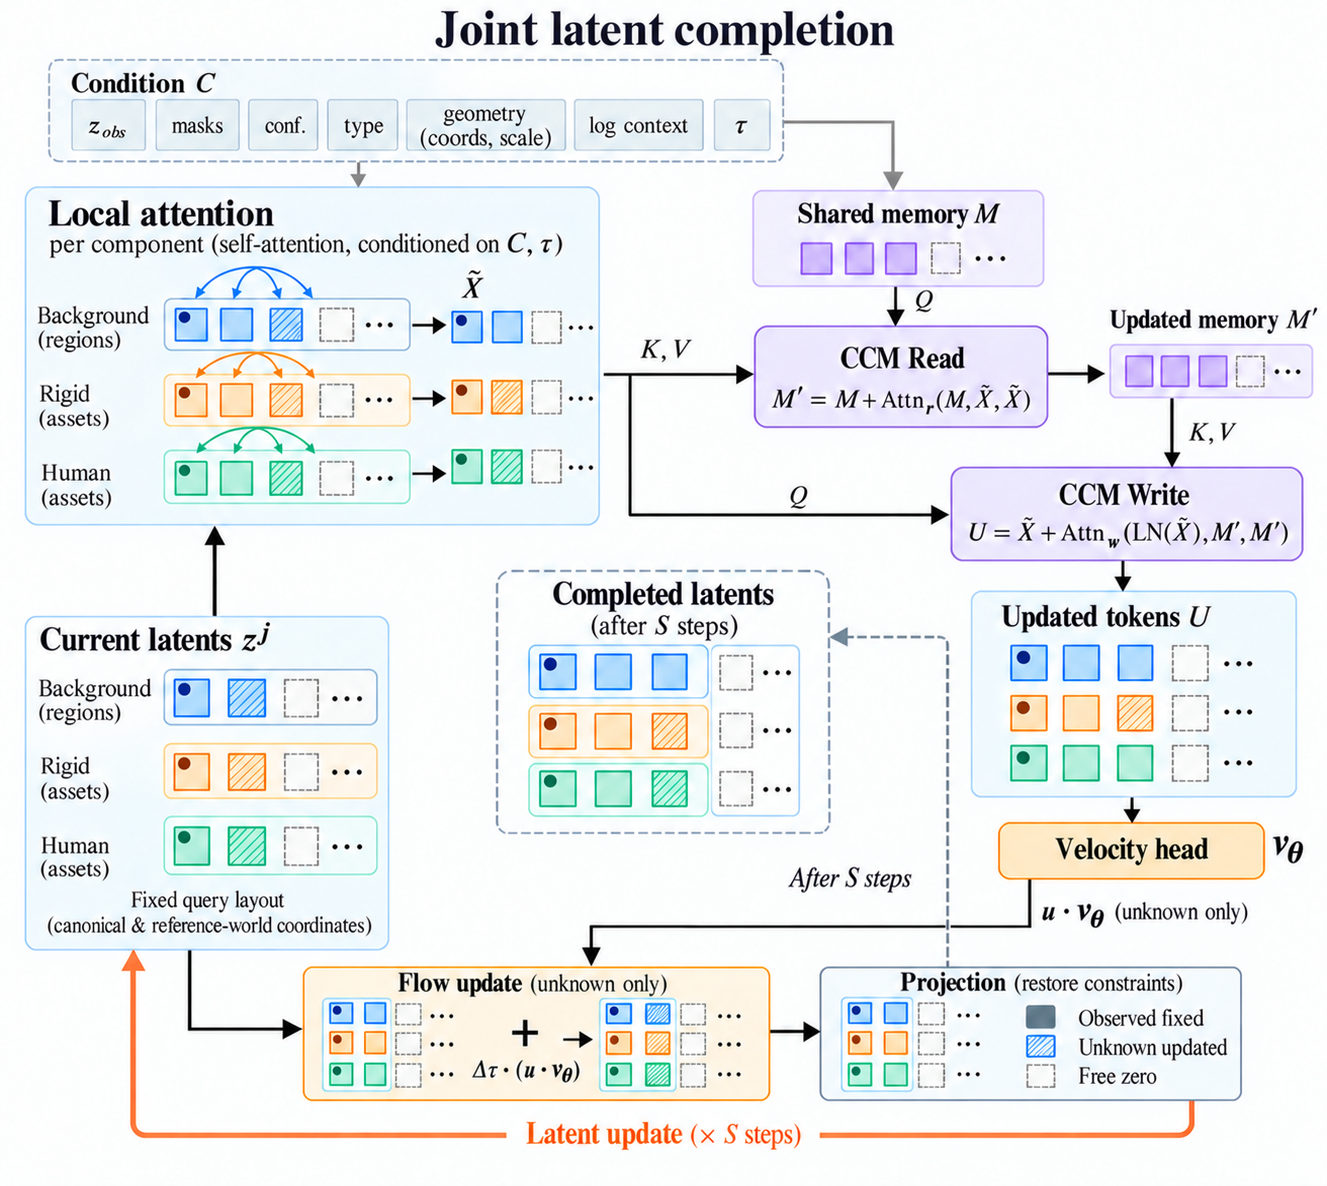
\includegraphics[width=0.86\textwidth]{../fig/drivecompose-joint-completion.png}
\caption{Enlarged version of the main joint-completion diagram. CCM reads group-local features into shared memory and writes context back. The velocity head and projection update unknown codes while restoring observed codes and clearing free-space codes.}
\label{fig:supp-detail}
\end{figure*}
